\documentclass{article}
\usepackage[round,sort]{natbib}
\usepackage{amsmath,amssymb,amsthm,amsfonts,hyperref, fullpage, setspace}
%\usepackage{easylist}%%%%%%%%%%%%%%%%%%%%%%%%%%%%%%%%%%%%%%%%%%%%%%%%%
\hypersetup{colorlinks=black,citecolor=black,pdfstartview=FitH, pdfpagemode=None}
\usepackage{eucal}
\usepackage{booktabs}
\usepackage{dcolumn}
\usepackage{sectsty}
\usepackage{subeqnarray}
\usepackage[utf8]{inputenc}
\usepackage{graphicx,psfrag} %only include if using pictures
\usepackage{color}
\usepackage{pdfpages}
\usepackage{ifthen} %only include if using conditional package
\usepackage{sectsty}
\usepackage{subfig}
\usepackage{float}
\usepackage[T1]{fontenc}
\usepackage{booktabs}
\usepackage[english]{babel}
\usepackage{geometry}
\usepackage{graphicx}
\usepackage{longtable}
\usepackage{afterpage}
\usepackage{pdflscape}
\usepackage{float}
\usepackage{lipsum}
\usepackage[colorinlistoftodos]{todonotes}

 \geometry{
 a4paper,
 total={170mm,257mm},
 left=35mm,
 right=35mm,
 top=34mm,
 bottom=34mm
 }
 
\linespread{1.6} 
\newcommand{\B}{\bf}
\newtheorem{thm}{Theorem}

\newtheorem{defn}[thm]{Definition}

\newtheorem{lemma}[thm]{Lemma}

\newtheorem{claim}[thm]{Claim}

\newtheorem{proposition}[thm]{Proposition}

\newtheorem{conjecture}[thm]{Conjecture}

\newtheorem{corollary}[thm]{Corollary}

\newtheorem{remark}[thm]{Remark}
\newcommand{\hhs}[1]{\hspace{#1mm}}
\newcommand{\hs}{\hspace{5mm}}
\newcommand{\vp}{\vspace{1mm}}
\newcommand{\vs}{\vspace{5mm}}
\newcommand{\jl}{$\frac{}{}$} %User defined for empty symbol to jump line
% ********************** newcommand *********************************
\newcommand{\mbf}[1]{\mbox{\boldmath $#1$}}
\newcommand{\hb}[1]{\hspace{-#1 mm}}
\newcommand{\ds}{\displaystyle}
\newcommand{\QED}{\hfill $\Box$}
% *********************** frequently used math symbols from AMS *******
\newcommand{\norm}[1]{\left\Vert#1\right\Vert}
\newcommand{\abs}[1]{\left\vert#1\right\vert}
\newcommand{\set}[1]{\left\{#1\right\}}
\renewcommand{\arraystretch}{1.5}
\newcommand{\n}{\nabla}
\newcommand{\Hv}{\mathcal{H}_v}
\newcommand{\h}{\mathcal{H}}
\newcommand{\Ov}{\mathcal{O}_v}
\newcommand{\R}{\mathbb{R}}
\newcommand{\Rn}{\mathbb{R}^n}
\newcommand{\C}{\mathbb{C}}
\newcommand{\Cn}{\mathbb{C}^n}
\newcommand{\Z}{\mathbb{Z}}
\newcommand{\p}{\partial}
\newcommand{\ep}{\epsilon}
\newcommand{\eps}{\varepsilon}
\newcommand{\finv}{f^{-1}}
\newcommand{\im}{\imath}
\newcommand{\ga}{\gamma}
\newcommand{\fee}{\varphi}
\newcommand{\noi}{\noindent}
\newcommand{\bO}{\Omega}
\newcommand{\bX}{\mathbb{X}}
\newcommand{\bA}{\mathbb{A}}
\newcommand{\Oint}{\int_{\bO}}
\newcommand{\OXint}{\int_{\bO\times\bX}}
\newcommand{\Aint}{\int_{\bA}}
\newcommand{\Xint}{\int_{\mathbb{X}}}
\newcommand{\XXint}{\int_{\mathbb{X}^2}}
\newcommand{\E}{\mathbb{E}}
\newcommand{\pa}{\partial}
\newcommand{\tab}{\hspace*{2em}}
%\numberwithin{equation}{section}
 
\begin{document}

\title{\bf {\large ECO 395M: Time Series Econometrics}\vspace{1cm} \\
{\Large Rising Inflation and Taylor Rule in Turkey (2002-2020)}
\vspace{2cm}\\
{\Large THE UNIVERSITY OF TEXAS AUSTIN}\\
\begin{figure}[h!]
\centering 
\includegraphics[width=2.2in]{ut1.png}
\end{figure}
by
}

\author{Student: Lutfi Sun \\ 
        Instructor: Dr. Anastasia Zervou \\ 
        }

\date{\today}

\linespread{1.8}

\maketitle
\newpage
\tableofcontents
\newpage

\section{Introduction}

    Year-to-year percent change in Consumer Price Index has been above ten percent in Turkey since 2017. Coupled with the ever-continuous devaluation of Turkish Lira against the dollar and euro, the Turkish Economy is currently in a very concerning place. In this project, I study how the government responded to the rising inflation rates and what policies might have contributed to its rise and the devaluation of Turkish Lira in the first place.

    \begin{figure}[H]
        \centering
        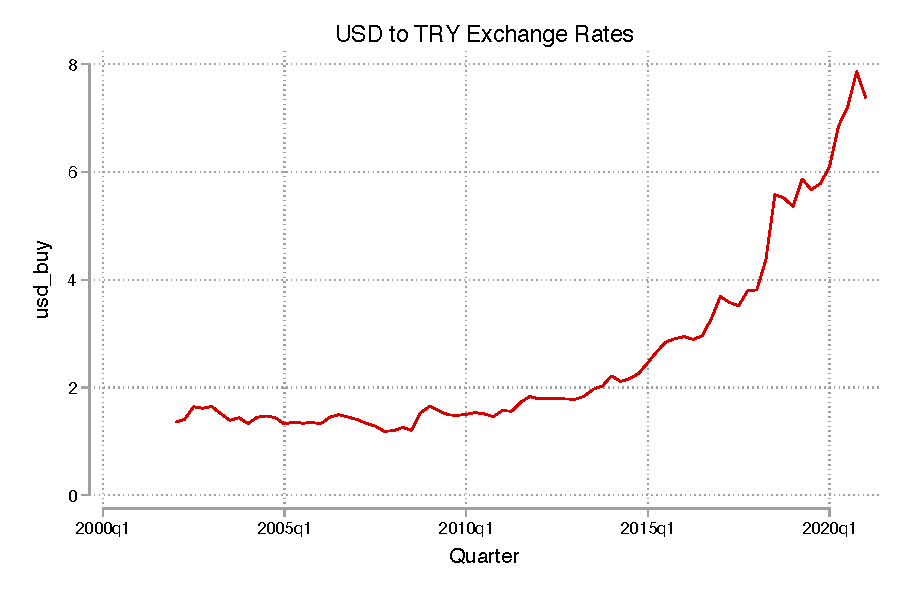
\includegraphics[width=\linewidth-1cm]{turkey_taylor/usd_fx_rates.pdf}
    \end{figure}

\subsection{Background}

    The political instability in Turkey in the 1990s brought a lack of trust in the government, large budget deficits, and foreign disinvestment. IMF issued a warning for financial crisis in 1996 and agreed to loan Turkey \$11.4 billion in 2000 (BBC, 2000). The loan was insufficient, and the government's actions could not stop the stock market crash. Interest rates and inflation kept rising while tens of thousands lost their jobs.
    \\ \\
    In February 2001, the Central Bank of Republic of Turkey (CBRT) and the government made a joint decision to implement a floating exchange rate regime. Soon after, the government adopted the Program of Transition to a Strong Economy and passed an amendment to the Central Bank Law. This gave CBRT more authority and independence to implement monetary policy.
    \begin{figure}[H]
        \centering
        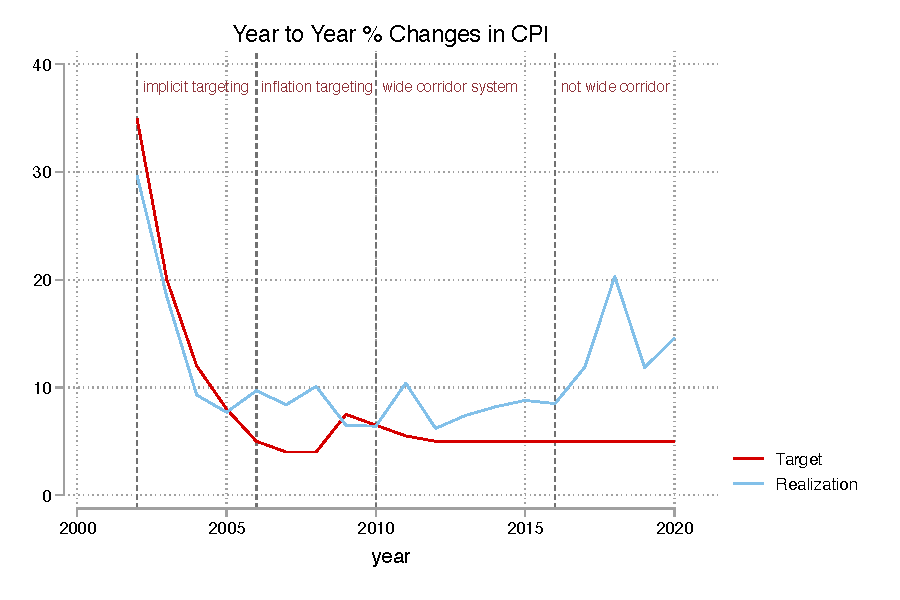
\includegraphics[width=\linewidth]{turkey_taylor/cb_inflation.pdf}
    \end{figure}
    {\setstretch{0.1}\tiny .}\\
    The following three years (2002-2005) is referred to as Implicit Inflation Targeting Period where the CBRT announced inflation targets jointly with the Turkish Government. In 2006, the Monetary Policy Committee received full authority over interest rates, began meeting on a monthly basis, and made meeting notes accessible to public. All these measures, along with other structural changes in fiscal policy, led to lower inflation and a more stable Turkish Economy.
    \\ \\
    Following the 2008 Global Financial Crisis, CBRT introduced new monetary policy tools such as reserve options mechanism, required reserve coefficient, and wide corridor system. After 2016, the Bank fixed the gap in the lending and borrowing rates citing that it "makes it difficult to understand the monetary policy stance" (TCMB).
    
    \begin{figure}[H]
        \centering
        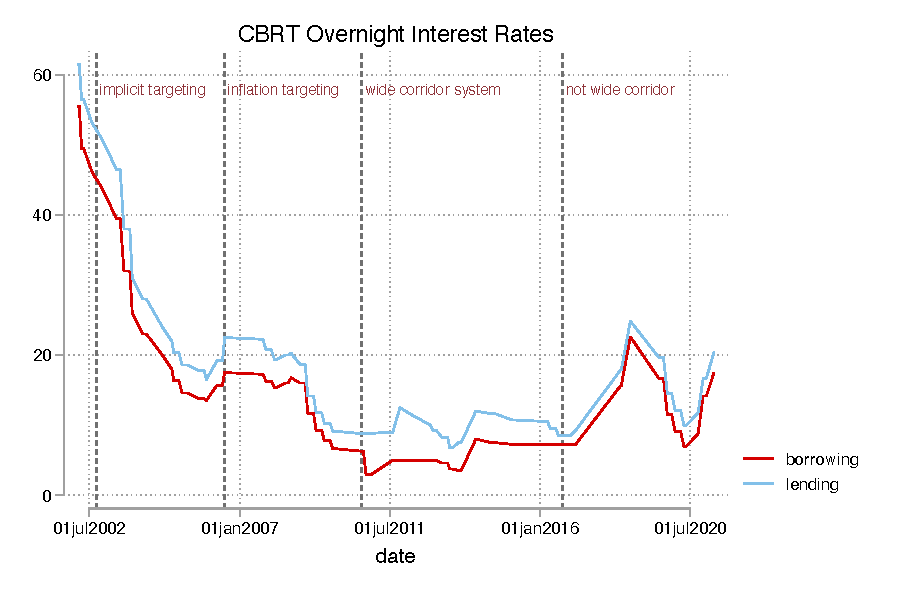
\includegraphics[width=\linewidth]{turkey_taylor/cb_oni.pdf}
    \end{figure}

\section{Data}

    I have gathered data from the Ministry of Treasury and Finance, TurkStat, and Central Bank of Turkey:
    \begin{itemize}
        \item https://www.hmb.gov.tr/hmb-veri-dagitim-sistemi
        \item https://www.tuik.gov.tr/
        \item https://www.tcmb.gov.tr/
    \end{itemize}
    {\setstretch{0.1}\tiny .}\\
    My variables include: CBRT overnight interest rates, Consumer Price Index, Producer Price Index, Gross Domestic Product, USD-TRY Exchange Rates, Borsa Istanbul Volume, Foreign Direct Investment, and more. The observations go from the first quarter of 2002 to the first quarter of 2021 (2020 Q4 for some).
    \begin{figure}[H]
        \centering
        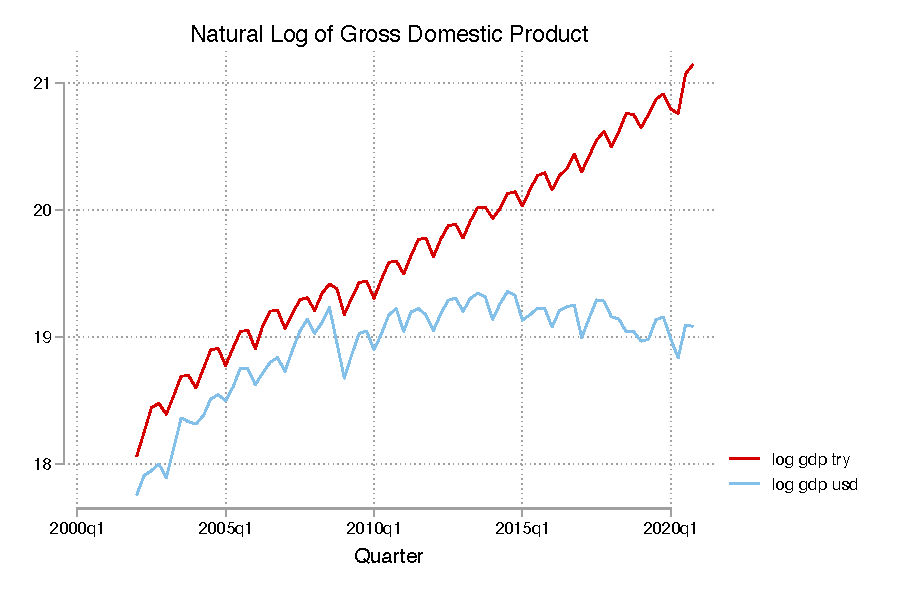
\includegraphics[width=\linewidth-1cm]{turkey_taylor/gdp.pdf}
    \end{figure}
    I define output gap in two ways. First, I transform the GDP to its natural log form and take the residuals from an OLS regression with trend and quarter dummies. The other way is I deseaonalize the OECD's Composite Leading Indicator (CLI) which is designed to "provide early signals of turning points in business cycles" (OECD 2021). I report the results from the former in this paper. Please see the comments and labels in the provided Do-File for more information on data and transformation.

    \begin{figure}[H]
        \centering
        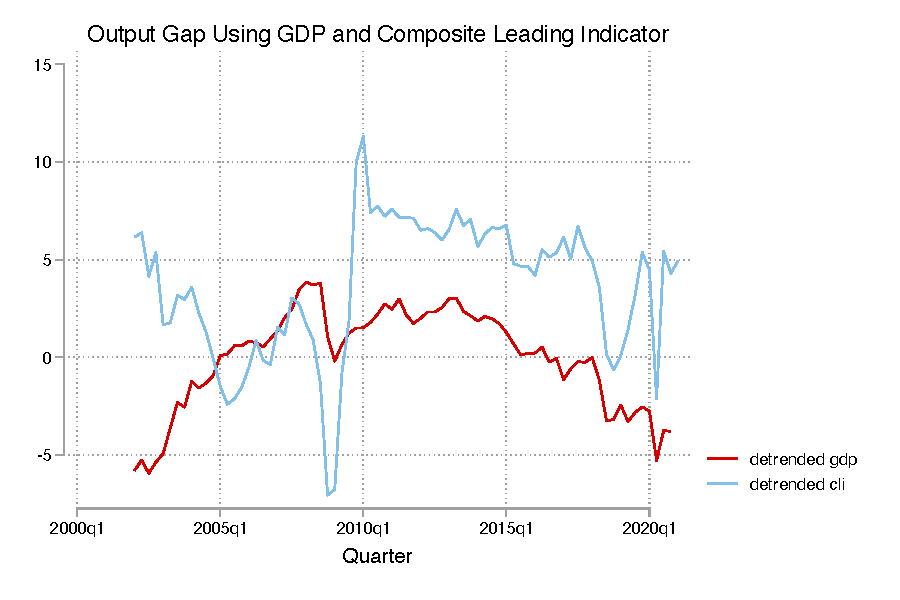
\includegraphics[width=\linewidth-1cm]{turkey_taylor/output_gap.pdf}
    \end{figure}
\section{Model Estimation and Results}

    $$i_{t}=\pi_{t}+r_{t}^{*}+a_{\pi}\left(\pi_{t}-\pi_{t}^{*}\right)+a_{y}\left(y_{t}-\bar{y}_{t}\right)$$
    {\setstretch{0.1}\tiny .}\\
    Following the literature, I try to estimate the Taylor Equation and take the overnight borrowing rate to be the policy variable. However, it is important to note that CBRT has multiple rates in its toolbox as discussed above.
    
\subsubsection{Short-Run Structural Vector Auto-Regressive Model}

    For short-run SVAR, I assume inflation has no contemporaneous effect on output gap and that it takes at least a quarter for Central Bank policy to influence inflation and output. 
    
    $$
    \begin{aligned}
    \Delta lny_{t} &= \alpha_{1}+\beta_{12} \pi_{t}+ \beta_{13} i_{t} + \gamma_{11} \Delta lny_{t-1} + \gamma_{12} \pi_{t-1} + \gamma_{13} i_{t-1} + \cdots +  \varepsilon_{1 t}\\ 
        &= \alpha_{1} + \gamma_{11} \Delta lny_{t-1} + \gamma_{12} \pi_{t-1} + \gamma_{13} i_{t-1} + \cdots +  \varepsilon_{1 t}\\
    \pi_{t} &= \alpha_{2} + \beta_{21} \Delta lny_{t} + \beta_{23} i_{t} + \gamma_{21} \Delta lny_{t-1} + \gamma_{22} \pi_{t-1} + \gamma_{23} i_{t-1} + \cdots + \varepsilon_{2 t}\\
        &= \alpha_{2} + \beta_{21} \Delta lny_{t} + \gamma_{21} \Delta lny_{t-1} + \gamma_{22} \pi_{t-1} + \gamma_{23} i_{t-1} + \cdots + \varepsilon_{2 t}\\
    i_{t} &= \alpha_{3} + \beta_{31} \Delta lny_{t} + \beta_{32} \pi_{t} + \gamma_{31} \Delta lny_{t-1} + \gamma_{32} \pi_{t-1} + \gamma_{33} i_{t-1} + \cdots +\varepsilon_{2 t}
    \end{aligned}
    $$ 
    
    In matrix notation,
    $$
    \left[\begin{array}{lll} 1 & 0 & 0 \\ -\beta_{21} & 1 & 0 \\ -\beta_{31} & -\beta_{32} & 1\end{array}\right] \left(\begin{array}{l} \Delta lny_{t} \\ \pi_{t} \\ i_{t} \end{array}\right) =  \left(\begin{array}{l}\alpha_{1} \\ \alpha_{2} \\\alpha_{3} \end{array}\right) + \sum_{i=1}^{8} A_{i} z_{t-i} + \varepsilon_{t}
    $$        
    $$
    Bz_{t} = \alpha + \sum_{i=1}^{8} A_{i} z_{t-i} + \varepsilon_{t}
    $$

\begin{figure}[H]
    \centering
    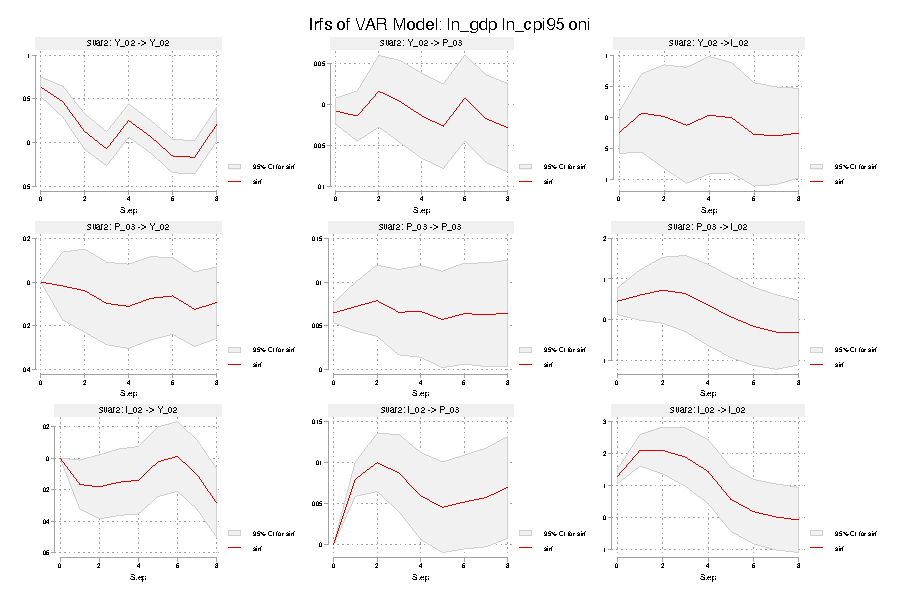
\includegraphics[width=\linewidth-2cm]{turkey_taylor/svar2.pdf}
\end{figure}
    {\setstretch{0.1}\tiny .}\\
    I find that shocks to output leads to higher prices and the effect is persistent. This would imply the growth we observe in Turkey in the past two decades is mostly demand-driven. Furthermore, shocks to Overnight Borrowing Rates lead to higher and persistent rises in inflation. This is contradictory with the standard theory and an example of price puzzle. CBRT seems to responds to growing economy by reducing rates (at least in the first few quarters). This is at odds with what standard macroeconomic theory would suggest the bank to do: contractionary policy during booms. Below is a figure of Cumulative IRFs from Long Run SVAR model.
    
    
\begin{figure}[H]
    \centering
    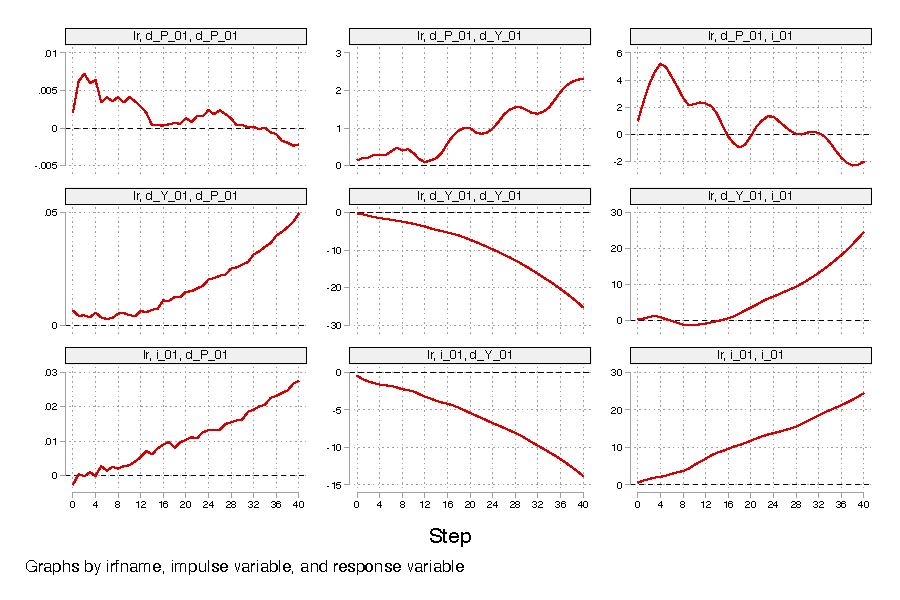
\includegraphics[width=\linewidth-2cm]{turkey_taylor/lvar_cumulative.pdf}
\end{figure}

\subsubsection{SVAR Including Exchange Rates}

    In this model, I do not convert the output levels to dollar and keep them in terms of nominal Turkish Lira. Instead, I include USD/TRY exchange rates in the model. In order to combat the price puzzle, I use producer price index instead of CPI as a measure of inflation.

\begin{figure}[H]
    \centering
    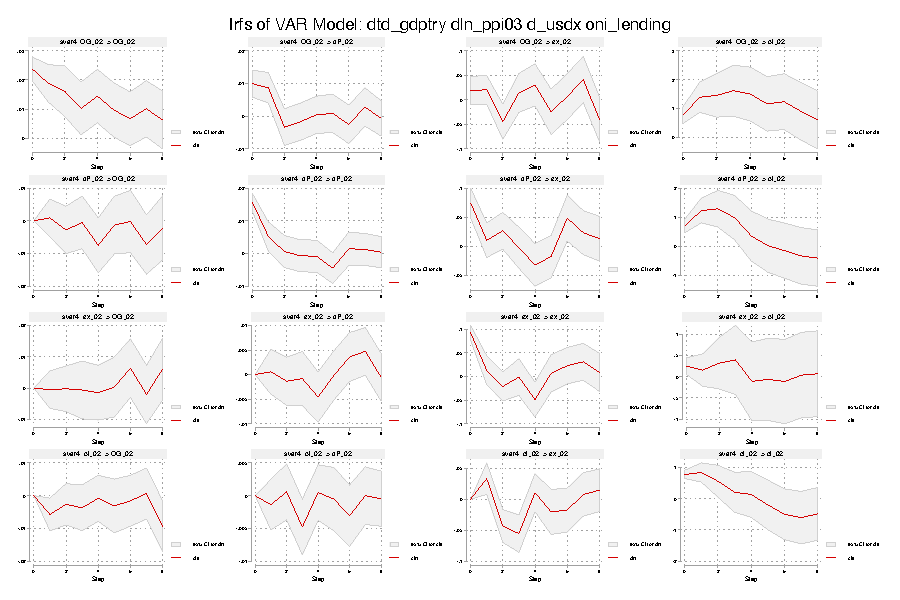
\includegraphics[width=\linewidth]{turkey_taylor/svar4_try.pdf}
\end{figure}
    {\setstretch{0.1}\tiny .}\\
    We see that a rise in CBRT interest rate does not lead to higher prices (no more price puzzle). A shock to the value of US Dollar against Turkish Lira eventually increases inflation. And a shock to overnight lending rates lowers the exchange rate in the second and third quarters that follow. 
    \\ \\
    We also observe CBRT to be responding to growth more inline with theory by increasing interest rates (at least for six quarters). Furthermore, the CBRT tries to fight inflation by also increasing interest rates for about four quarters.
    \\ \\
    In my further studies on this subject, I plan to have monthly data and analyze these decades in three parts: 2002-2010, 2011-2016, 2016-2021. I also want to utilize Kalman Filter to better understand and show how the ways the Central Bank interpreted the economy and responded to its shocks have evolved.

\newpage
\section{References}

    \begin{enumerate}
    
        \item Alkan, Buket. Journal of Economics and Political Economy; Istanbul Vol. 6, Iss. 1,  (Mar 2019): 78-93. DOI:10.1453/jepe.v6i1.1851 
        \item Kara, Hakan, Ogunc, Fethi and Sarikaya, Cagri, (2017), Inflation Dynamics in Turkey: A Historical Accounting, CBT Research Notes in Economics, Research and Monetary Policy Department, Central Bank of the Republic of Turkey.
        \item BBC News. “IMF Agrees Turkish Loans.” , BBC, 6 Dec. 2000, news.bbc.co.uk/2/hi/business/1057382.stm. 
        \item Khakimov, O.A. Erdogan, Levent Cağlarirmak, Necla. (2010). Assessing monetary policy rule in Turkey. International Journal of Economic Perspectives. 4. 319-330.
        \item OECD. “Leading Indicators - Composite Leading Indicator (CLI)" OECD Data, data.oecd.org/leadind/composite-leading-indicator-cli.htm. 
        \item TCMB. Central Bank Monetary Policy Framework.\\ www.tcmb.gov.tr/wps/wcm/connect/EN/TCMB+EN/Main+Menu/Core+Functions/Monetary+Policy/Central+Bank+Monetary+Policy+Framework. 


    \end{enumerate}

\end{document}
